\documentclass{article}

\usepackage{neurips_2026}
\usepackage[utf8]{inputenc}
\usepackage[T1]{fontenc}
\usepackage{hyperref}
\usepackage{url}
\usepackage{booktabs}
\usepackage{amsfonts}
\usepackage{amsmath}
\usepackage{nicefrac}
\usepackage{microtype}
\usepackage{xcolor}
\usepackage{graphicx}

% Paths are relative to tex/. Both figures this draft includes live in figures/splicebert/.
\graphicspath{{../figures/splicebert/}{../figures/splicebert/workshop_edits/}{../figures/origin-crossmodel/}}

\title{Causal Mechanistic Discovery in Genomic Foundation Models}

\author{%
  Cameron Berger\\
  Algoverse\\
  Address\\
  \texttt{email}
}

\newcommand{\Uinfo}{\ensuremath{U_{\mathrm{info}}}}

\begin{document}

\maketitle

\begin{abstract}

\end{abstract}
\setcounter{section}{1}
\section{Introduction}

Foundation models for DNA and RNA span a multitude of designs: k-mer and BPE transformers, single-nucleotide masked models, long-convolution, and reverse-complement-equivariant state-space models \citep{ji2021dnabert,chen2024splicebert,zhou2024dnabert2,dallatorre2025nt,nguyen2023hyenadna,schiff2024caduceus}. These design choices limit both the mechanisms a model can learn and those researchers can test: tokenization determines spatial resolution, positional encoding constrains available addressing schemes, and architecture determines which internal variables can be intervened on.

Interpretation in genomics has produced genuine insights.  Input perturbations and local surrogate models recover motifs and syntax \citep{avsec2021bpnet,seitz2024squid}; attention and representation analyses relate GFM components to annotated elements \citep{ji2021dnabert,chen2024splicebert,dallatorre2025nt,consens2025genomicattention}.  These approaches ask which sequence features affect a prediction, or which internal states associate with known annotations.  We ask a complementary question: \emph{how does a frozen GFM implement a predefined, model-native biological computation?}

We present three distinct contributions. First, we formalize an evidence ladder for GFM mechanistic discovery, connecting causal abstraction and component-level interventions, to biological claims \citep{elhage2021framework,geiger2025causal,zhang2024patching}. Second, we use it to resolve implementation of acceptor-donor coupling computation in SpliceBERT. Third, we show [TODO: DNABERT-2 contributions]. In our analysis, we report failed gates and retracted claims alongside positive results as these outcomes rule out candidate mechanisms and clarify the limits of the evidence.

\section{Methodology}
\label{sec:methods}

\subsection{Biological Computation to Model-Native Behavior}
\label{sec:comp-behavior}

We start with a known biological computation that can be operationalization through a model's output. For SpliceBERT, the candidate computation is conditional donor-acceptor recognition and the readout is masked-donor nucleotide margin. We must first establish that the assay can distinguish the causal effect from an artifact. A positive control must produce an expected effect, showing the assay is sensitive to the mechanism being studied. A matched negative control must remain near zero, bounding changes caused by the intervention procedure. Planted-effect tests must recover the effects, establishing the assay's resolution. Identity interventions must leave the model's output unchanged, checking that patching, indexing, and bookkeeping are correct. Health metrics show that the intervention has not damaged the model. We freeze the assay, thresholds, and analysis plan only after all five families pass; otherwise, the target result is treated as uninterpretable.

\begin{table}[t]
  \caption{\textbf{Evidence ladder.} Each rung answers a different question. }
  \label{tab:ladder}
  \centering
  \small
  \setlength{\tabcolsep}{4.5pt}
  \begin{tabular}{p{0.18\linewidth}p{0.39\linewidth}p{0.31\linewidth}}
    \toprule
    Level & Question & Evidence\\
    \midrule
    Behavior & Does the model perform a selective computation?& Matched corruption;
    native margin \\
    Representation & Is a candidate feature present? & Probe, geometry, spectrum \\
    QK / selection & Can it change source selection? & QK decomposition; K/Q exchange \\
    Attention & Is routing changed after softmax? & Pattern intervention \\
    OV / mediation & What is written, and along which path? & V/OV exchange; path or subspace patch \\
    Faithfulness & Can the proposed computation regenerate the behavior?& Complement scrub; size curve \\
    Biology & Is there independent evidence for a biological process?& External assay; natural experiment\\
    \bottomrule
  \end{tabular}
\end{table}
Table~\ref{tab:ladder} separates position/representation, selection, routing, value writing, mediation, behavior, and biological interpretation.  This is a scoped causal abstraction: an interpretation maps network variables to an algorithm and tests the map with corresponding interventions \citep{geiger2025causal}.  Automated pruning and edge scoring can scale candidate generation \citep{conmy2023acdc,syed2024eap}, but computational preservation and completeness remain empirical questions \citep{wang2023ioi,mueller2025mib}.

\section{SpliceBERT: A Paired-Site Computation}
\label{sec:splicebert}

\subsection{Definitions}

SpliceBERT is a six-layer, 16-head, single-nucleotide masked language model trained on primary RNA from 72 vertebrates \citep{chen2024splicebert}.

Internal exons were drawn from GENCODE v50 on GRCh38 \citep{mudge2025gencode}. Each example is a 1024-nt genomic window in transcript orientation. For the relevant study, upstream acceptor offset is deterministically randomized over 100--300 n. We exclude ambiguous sequence, non-canonical splice motifs, assembly-boundary crossings, and exons outside 20--500 nt. Gene-disjoint splits assign chr11/16/19 to validation and chr8/9 to sealed test. The principal coupling cohort contains canonical downstream introns of 60--150 nt.

At the masked \(\mathrm{G}\) of a donor \texttt{GT}, the native MLM margin is
\begin{equation}
  m(\mathbf{x};d)
  =
  \ell_{\mathrm G}(\mathbf{x};d)
  -
  \max_{b\in\{\mathrm{A,C,T}\}}\ell_b(\mathbf{x};d).
  \label{eq:margin}
\end{equation}
The matched corruption replaces the annotated downstream acceptor \texttt{AG} with \texttt{CC}. Donor--acceptor coupling is the change in the masked-donor margin caused by the acceptor corruption, defined as
\begin{equation}
  C_{\mathrm{intron}}
  =
  m(\mathbf{x}^{N};d)-m(\mathbf{x}^{D^-};d),
  \label{eq:coupling}
\end{equation}
where \(N\) and \(D^-\) denote intact and acceptor-corrupt sequence. The edit is length preserving and changes only the acceptor di-nucleotide. Behavioral effects use the unconditional cohort. Normalized recovery uses a prespecified mechanism cohort with \(C_{\mathrm{intron}}\geq0.3\).

Factorial and difference-in-differences analyses use the linear margin
\begin{equation}
  m^{\mathrm{lin}}(\mathbf{x};d)
  =
  \ell_{\mathrm G}(\mathbf{x};d)
  -
  \frac{1}{3}\sum_{b\ne\mathrm G}\ell_b(\mathbf{x};d).
  \label{eq:linear-margin}
\end{equation}
Margin, coupling, and their intervention effects are in logit units; nats are reserved for cross-entropy damage.

\subsection{Circuit Interventions}
\label{sec:circuit-methods}

Exhaustive head scans, position and residual geometry, QK decomposition, attention, and Fourier spectra generated candidates. Candidate statistics did not enter causal claims without intervention. We separated position-table presence, pre-softmax QK selection, post-softmax routing, OV or behavioral mediation, and native behavior.

Coarse necessity replaced selected head outputs by dataset means and compared the loss with distinct size-matched random sets. Directed tests exchanged clean and corrupt queries, keys, values, attention patterns, head outputs, MLP outputs, position components, or residual subspaces. Clean-to-corrupt replacement measured denoising; corrupt-to-clean replacement measured necessity. Masked-base MLM accuracy served as a health control. Activation replacement followed paired patching practice \citep{zhang2024patching,
heimersheim2024patching}; selection and value writing were analyzed separately
\citep{elhage2021framework}.

For L3H1 at donor query \(d\), head output is \(Z_d=\sum_j A_{dj}V_j\). We cached \(A_N,A_D,V_N,V_D\), reconstructed \(Z(A,V)=AV\), and injected each cell of the \(2\times2\) attention--value factorial into a common downstream run. Address-only, payload-only, and joint recovery were therefore evaluated on the same output computation. Exact reconstruction, identity injection, and value linearity were required preflight checks.

The donor-side readout subspace \(\Uinfo\) is the leading left-singular subspace of the clean-minus-corrupt final residual at the masked donor. Bases were estimated on one gene subset and evaluated on another. Sufficiency added the clean rank-\(k\) component to the corrupt residual; necessity removed or replaced it reciprocally. Nulls matched rank and activation energy. We use \(\Uinfo\) as an operational label, not a semantic assignment \citep{makelov2024subspace}.

For a node set \(S\), denoising \(D(S)\) is the recovered fraction after injecting clean node outputs into the corrupt run; necessity \(N(S)\) is the fraction destroyed by the reciprocal intervention. Complement faithfulness \(F(S)\) keeps \(S\) clean while replacing every measured node outside \(S\)with its matched corrupt activation. Ratios use mean clean--corrupt effects with gene-bootstrap intervals. A static backward-removal ranking over 96 heads, six MLPs, and the embedding was evaluated on held-out genes at 17 sizes. Because nodes were not re-ranked after each removal, the curve upper-bounds the smallest set found by this search and does not establish minimality.

\subsection{Positional Carriers}
\label{sec:carrier-methods}

We centered each learned position matrix and decomposed its position axis into Fourier sine/cosine subspaces. Carrier interventions projected out a candidate band, restored it at selected positions, or scaled its dose. Control bands matched rank, geometry, and removed energy.

Period-3 use was tested independently by nucleotide-invariant local surgery. The learned hidden direction was shifted in register by 3, 6, or 9 nt or off register by adjacent offsets, without changing sequence tokens, coordinates, motifs, or length. The primary contrast compared modulo recovery in coding-sequence (CDS) blocks with the identical surgery in upstream intron blocks. Nineteen pre-seeded hidden-axis controls preserved the spatial waveform, Fourier support, Gram matrix, row norms, block geometry, and perturbation RMS.

The \(\simeq10.63\)-nt analysis used the stage-1 sibling pair. Reader tests required position-band mass, head-specific permutation significance with BH-FDR over the scanned family, post-softmax coherence, collapse after target carrier deletion, and retention under reciprocal-band deletion, low-leak-band deletion, and content shuffling. Sibling position spectra used
the same leakage-aware estimator. A 60-Mb human-genome spectrum and powered
position-table tests in RNA-FM and RNA-BERT assessed whether either carrier was
a universal sequence or genomic-MLM feature.

\subsection{Intervals and Permutations}
\label{sec:inference}

Intervals resample genes while preserving within-example pairing. Matched or source--target analyses use two-way gene-dyadic resampling. Permutation tests report
\begin{equation}
  p_{\mathrm{perm}}=\frac{H+1}{B+1},
\end{equation}
where \(H\) is the number of null statistics at least as extreme as the target among \(B\) permutations. Null families are matched to intervention size and geometry and are not pooled across sizes. Multiplicity is corrected over the executed scan. Each result records checkpoint, data, parameters, seed, command, code revision, and source hashes.

\subsection{SpliceBERT Results}
\label{sec:core}

On sealed chr8/9 genes with 60--150-nt downstream introns (\(n=400\)), acceptor corruption changes the donor margin by \(+0.872\;[0.771,0.969]\).  Matched non-partner \texttt{AG} and other-donor controls are \(+0.007\) and \(+0.005\) respectively. Thus the model has a selective paired-site dependency.

Mean-ablation of L3H1 and L2H15 removes 81.6\% of conditional coupling while retaining 99.2\% of masked-MLM health; the loss
exceeds all 400 distinct size-matched two-head nulls (add-one \(p=0.0025\)).

The 96-head scan identified L3H1 and L2H15 as the dominant necessary pair. Joint ablation removed 81.6\% of conditional coupling while retaining 99.2\% masked-MLM accuracy. Held-out denoising ranked L3H1 first, \(0.830\ [0.654,0.994]\), and L2H15 second, \(0.515\ [0.396,0.625]\).

At L3H1, address-only and payload-only reconstruct--inject recoveries are \(+0.01\) and \(+0.05\), whereas their joint intervention recovers \(+0.365\;[0.328,0.399]\).  The address is dominated by relative position-embedding geometry, with a reproducible 15--19\% local-content component.  The payload is localized to a four-token acceptor window and is generated through \(\{\mathrm{L0H7,L0H12,L0H10}\}\!\rightarrow\!\mathrm{MLP0}\!\rightarrow\!\mathrm{MLP1}\!\rightarrow\!\mathrm{MLP2}\), with redundancy among early heads.  [TODO: fill with resolution] It is not explained by preregistered bulk or frequency-composition.  Its semantic identity remains unresolved.

L3H1 converts this acceptor-local state into a donor-side low-rank format, \Uinfo.  A cross-fitted rank-8 patch recovers approximately 0.92 of coupling versus at most 0.05 for matched random subspaces.  Restoring L3H1 recovers 0.83, of which 0.93 is conditionally mediated through\Uinfo{} at donor \(\pm5\).  L4H0, L4H2, and L5H11 transport this state to the readout.

\begin{figure}[t]
  \centering
  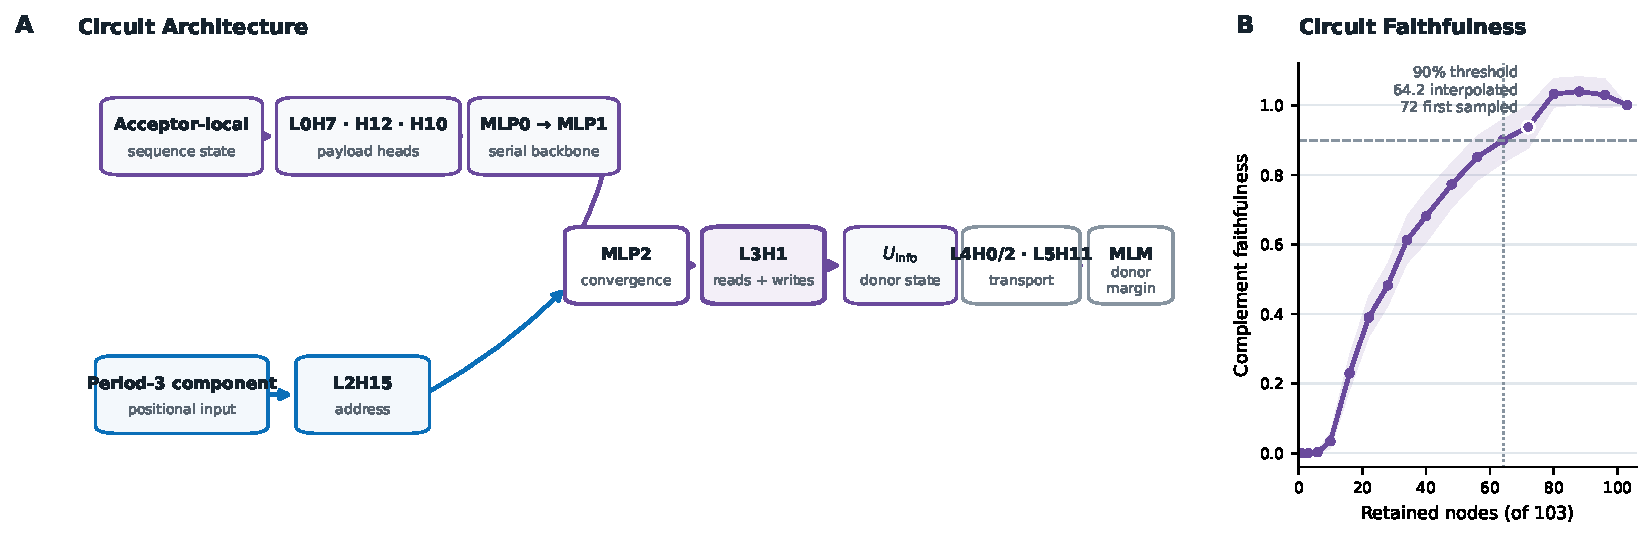
\includegraphics[width=\linewidth]{fig_full_circuit.pdf}
  \caption{\textbf{A }
  \textbf{A},x~\ref{app:artifacts}.}  \label{fig:core}
\end{figure}

The specified delivery spine destroys 98.9\% of coupling when corrupted and recovers \(0.986\;[0.982,0.991]\) when its clean outputs are injected.  Yet retaining the same nodes while scrubbing the complement preserves only \(0.005\;[0.003,0.008]\).  On held-out genes, 34, 56, 72, and 80 of 103 nodes reach 50, 80, 90, and 95\% complement faithfulness, respectively (Figure~\ref{fig:core}B).  A static ranking upper-bounds rather than proves the smallest faithful set.  The result rejects a sparse-circuit account while retaining a reproducible, top-ranked causal organization.

\subsection{Period-3 Carrier}
\label{sec:period3}

The final checkpoint contains a rank-2 period-3 position code. Period-3 deletion reduced donor coupling from \(0.946\) to \(0.027\); an energy-matched control retained \(0.944-0.953\). Restoring L2H15 or L3H1 after deletion recovered 0.363 and 0.348, above the matched one-head maximum of \(0.042\).

After removing the period-3 carrier, we restored it within progressively larger sequence windows. Donor or acceptor local restoration recovered only 2–4\% of lost coupling, while recovery approached one half at \(32\)nt. The carrier is therefore used across the donor–acceptor span rather than only at the splice-site boundaries.

We next separated L3H1’s attention pattern—where the head retrieves information, from its value vectors—the content retrieved. Restoring clean attention recovered \(+0.284 \ [0.192,0.386]\) raw logit units of coupling, whereas restoring clean values recovered none, \(-0.005\ [-0.013,0.003]\). The tested carrier effect therefore acts primarily by guiding L3H1’s routing.

\begin{figure}[t]
  \centering
  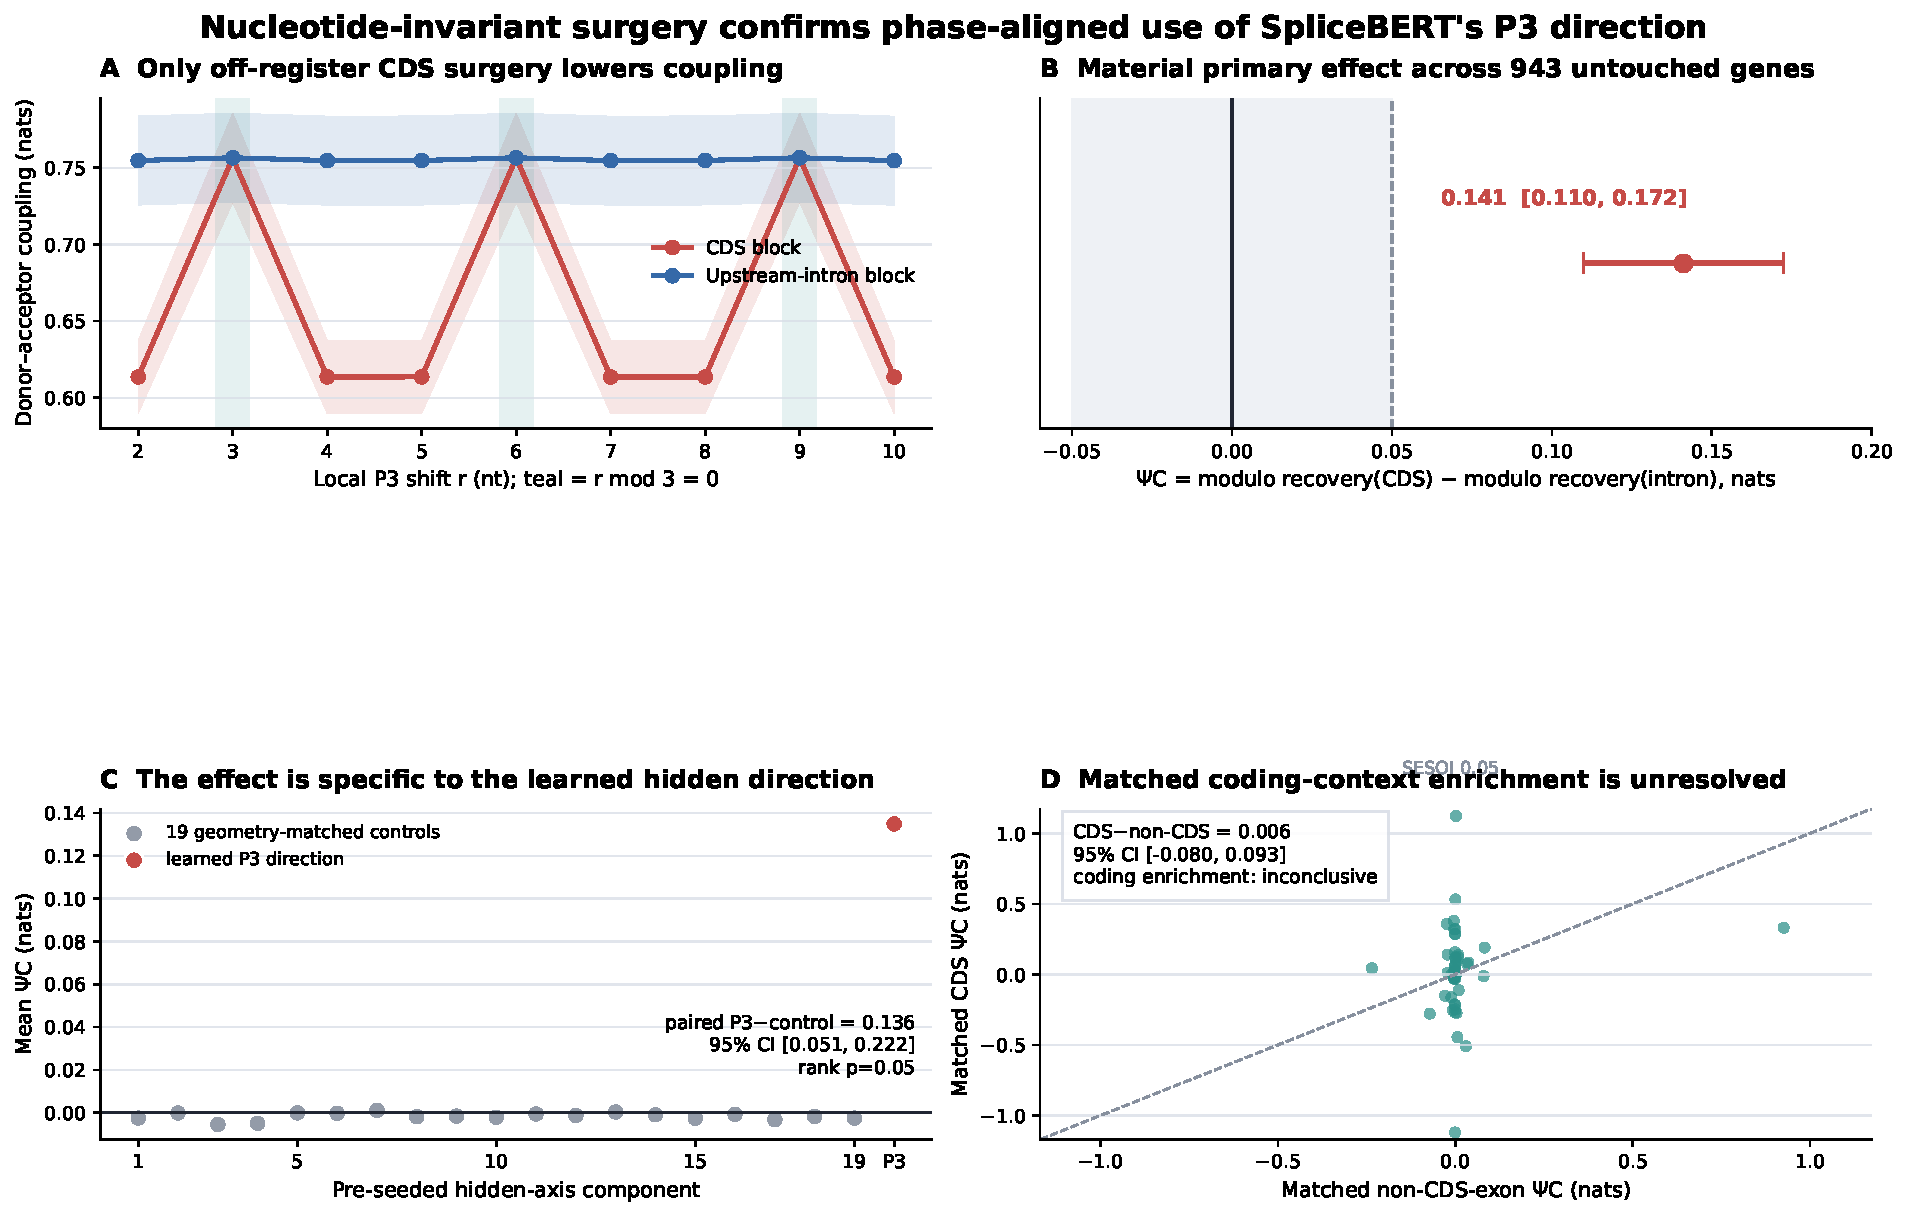
\includegraphics[width=\linewidth]{fig5_p3_phase_surgery_confirmation.pdf}
  \caption{\textbf{Clean}
  \textbf{A}, }  \label{fig:p3}
\end{figure}

A matched-checkpoint natural experiment separates present-day use from comparative corpus association. The 72-species and human-only checkpoints share architecture, stage, and 510-nt length.  Period-3 power is \(435\times\) versus \(6.2\times\) the median band; the latter is below a powered detection floor.  This associates the carrier with multi-species pretraining.  A sibling band-deletion result remains verification-level because only 12 controls qualify, fixing its exact add-one floor at \(1/13=0.077\).  Coding sequence is known to contain period-3 composition \citep{tiwari1997period3,yin2005fourier}, making codon periodicity a plausible corpus correlate, [TODO: fill in results of the experimental run]

\subsection{\texorpdfstring{\(\simeq10.63\)-nt}{10.63-nt} Carrier}
\label{sec:carrier10}

The multi-species position table contains a second carrier near \(10.63\)-nt, orthogonal to the period-3 plane. Eight heads passed the post-softmax reader criteria. Deleting the target carrier retained 27--44\% of their patterns; reciprocal-band deletion retained 89--97\%, low-leak-band deletion retained approximately 100\%, and content shuffling retained 93--107\%.

The tested downstream effects were small. Reader-value interventions were below the 0.02-logit-unit donor-coupling threshold, and carrier deletion changed coupling by \(-0.033\ [-0.061,-0.005]\). A general MLM-output diagnostic gave relative value-write scores of \(0.002\)--\(0.003\). These results bound the tested donor and general output paths. They do not establish absence of all downstream function.

The carrier was \(369\times\) the median band in the 72-species stage-1 checkpoint and \(2.4\times\), undetected, in the human-only sibling. No \(\simeq10.63\)-nt signal was detected in a 60-Mb human-genome spectrum or in the RNA-FM and RNA-BERT position tables. The model carrier is also distinct from the measured \(\simeq10.298\)-nt nucleosomal periodicity: the 0.33-nt gap is about seven times the larger measured wavelength spread. Thus the \(\simeq10.63\)-nt carrier is a corpus-attributed positional attention circuit with bounded downstream function.

\begin{table}[t]
  \caption{\textbf{Evidence boundary for the positional carriers.} Values from
  the final 1024-nt checkpoint and stage-1 sibling comparison are reported
  separately in the text.}
  \label{tab:carrier-evidence}
  \centering
  \small
  \begin{tabular}{lll}
    \toprule
    Level & Period-3 & \(\simeq10.63\) nt \\
    \midrule
    Position table & Rank-2 code& R-2 carrier\\
    Attention & L3H1 Routing& Eight Heads\\
    Donor behavior & Causal Support& Small Shift\\
    Corpus contrast & 435 vs 6.2\(\times\) & 369 vs 2.4\(\times\) \\
  \end{tabular}
\end{table}
\section{Biological Bridges, Refutations, and Scope}
\label{sec:biology}

\paragraph{Periodicity}


\section{Discussion}

The central result is methodological as much as anatomical.  In SpliceBERT, a behavior-first intervention workflow recovers a relative address and acceptor-local payload before a low-rank donor delivery state, while also exposing the computation's distributed faithfulness boundary. [TODO: Whether the workflow identifies a comparable or different organization in DNABERT-2 is left open pending the complete result package]

Three practices make that conclusion possible.  First, the model-native behavior is established before internal search.  Second, selection, attention, value writing, and behavior remain separate.  Third, failed gates constrain the claim: SpliceBERT's delivery spine is not a faithful sparse generator; [TODO: the period-3 code is...].

\paragraph{Limitations}
The complete mechanistic account concerns one frozen SpliceBERT checkpoint and a restricted short-intron cohort. Candidate search can miss redundant or nonlinear mechanisms, and a static removal ranking only upper-bounds the smallest faithful set.  Activation exchange probes local counterfactuals and may leave the model manifold.  Biological labels are external to the frozen-model causal graph, and
payload semantics are non-identifiable under the tested assays.  Corpus attribution compares published siblings but cannot isolate species diversity from corpus size, composition, or optimization.  Finally, the experiments audit existing models; they do not validate genomic predictions for clinical use or measure molecular function in cells.

\paragraph{Impact}
Stronger causal audits can reduce the risk of presenting attractive GFM features as biological discoveries and can expose architecture-induced artifacts before downstream use. Conversely, mechanistic labels may acquire unwarranted authority in biomedical settings.  We therefore report operational model variables, preserve refutations, and avoid mapping components to molecular actors without independent experiments.  No individual genomes, clinical records, human subjects, or model training are introduced in this work.

\section{Conclusion}

Mechanistic discovery in GFMs should begin with a selective model behavior and end at the highest evidence rung actually reached.  In SpliceBERT, that standard supports an address--payload--delivery mechanism inside an irreducibly distributed computation and a causal period-3 routing coordinate. The strongest licensed claim is a causal account of frozen-model computations.


\bibliographystyle{plainnat}
\bibliography{refs}

\newpage
%% NeurIPS 2026 Workshop Paper Checklist
%% Interpretability for Discovery Workshop

\section*{Paper Checklist}

\begin{enumerate}

\item \textbf{Claims.}
Do the main claims made in the abstract and introduction accurately reflect the paper's contributions and scope?
\answerYes{} The abstract and introduction present three specific claims (circuit structure, period-3 carrier, faithfulness) that are directly supported by the results in §3. Each claim is scoped to one checkpoint (SpliceBERT.1024nt), one task (masked donor prediction), and one behavioral assay (canonical short introns). No transfer to biological mechanisms or other models is asserted beyond what is measured.

\item \textbf{Limitations.}
Did you discuss the limitations of your work?
\answerYes{} §4 (Discussion) explicitly identifies three open questions: (a) the acceptor-payload semantic identity is unresolved and cannot be named on the current checkpoint; (b) the $\approx$10.63-nt carrier's OV function in the donor circuit is bounded at sub-SESOI levels and its general function is open; (c) cross-example specificity of the acceptor payload is not separable at current precision. §3.3 clarifies that the named circuit is a structured core within an irreducibly distributed computation, not a minimal sparse generator.

\item \textbf{Theory assumptions and proofs.}
If the paper includes theoretical contributions, do all theorems, corollaries, etc.\ appear to be correct?
\answerNA{} This paper contains no theoretical claims or proofs.

\item \textbf{Experimental reproducibility.}
Are the experimental results reproducible?
\answerYes{} All results are derived from the published SpliceBERT checkpoint (publicly available) and GENCODE v43 annotations (public). Code, preregistrations, and JSON result artifacts are included in the supplementary repository. Every claim is controlled by an immutable artifact file listed in the results manifest. Pre-registered protocols with smoke-gate tests and adversarial verification were used throughout.

\item \textbf{Code.}
Is code available, or will it be made available?
\answerYes{} The full analysis codebase will be released upon de-anonymization. The codebase includes all runner scripts, pre-registration documents, and result manifests.

\item \textbf{Compute.}
Does the paper include the compute required to reproduce the results?
\answerYes{} All experiments use a single pre-trained SpliceBERT checkpoint (inference only, no training). Compute requirements are modest: all analyses run on a single GPU in under 48 hours total. No large-scale compute is required to reproduce these results.

\item \textbf{Data.}
Does the paper reference all data used?
\answerYes{} The model (SpliceBERT.1024nt) is publicly available~\citep{chen2024splicebert}. Genomic annotations use GENCODE v43~\citep{mudge2023gencode}. RNA-FM and RNA-BERT checkpoints are publicly available~\citep{chen2022rnafm,akiyama2022rnabert}. The human-only SpliceBERT sibling checkpoint is publicly available from the same source as SpliceBERT.

\item \textbf{IRB approvals.}
If the paper involves human subjects, was ethical approval obtained?
\answerNA{} This paper involves no human subjects. All data are publicly available genomic annotations and pre-trained model weights.

\item \textbf{Responsible use.}
Does the paper discuss potential positive societal impacts, as well as any potential negative impacts?
\answerYes{} See below.

\end{enumerate}

\subsection*{Responsible Use Statement}

\paragraph{Potential positive societal impacts.}
This work develops mechanistic interpretability methods applicable to genomic foundation models. The methods — reconstruct--inject patching, position-table Fourier analysis, and nucleotide-invariant causal surgery — are designed to surface internal computations that are not accessible by behavioral probing alone. Positive impacts include: (1) improved understanding of what genomic models learn from multi-species pretraining data; (2) a transferable methodological template for auditing other GFMs for spurious or biologically meaningful features; (3) identification of open questions (e.g.\ acceptor-payload identity) that can guide future model evaluation and data collection.

\paragraph{Potential risks and mitigations.}
The methods described in this paper are interpretability tools applied to an existing published model; they do not enable training new genomic models or generating novel sequences. The primary risk is misinterpretation of results: (1) the donor--acceptor circuit is a model mechanism, not a direct claim about spliceosome biochemistry or transcript abundance; no external biological assay is used; (2) the period-3 carrier is attributed to multi-species pretraining by comparative analysis, not by retraining — origin dynamics cannot be recovered from a single checkpoint; (3) the faithfulness results show the named circuit is not a minimal sparse generator, and minimality is explicitly unclaimed. We have taken care throughout to scope claims precisely (see §3 and §4) and to avoid overstating biological implications. The open-source release of code and preregistration documents will allow independent verification and replication.

\paragraph{Broader context.}
Genomic foundation models are increasingly used in research and clinical genomics contexts. Mechanistic interpretability provides a tool for auditing these models before deployment, identifying features that may be spurious artifacts of training data rather than reflections of underlying biology. We view this work as a step toward model transparency in a domain where the stakes of misinterpreted predictions are high.


\end{document}
